\documentclass[14pt]{beamer}
\usetheme{Montpellier}
\usecolortheme{beaver}

\usepackage{amsmath, amssymb, ../../vimacros, hyperref, enumerate}
\usepackage[round]{natbib}

\usepackage{multicol}
\usepackage{physics}
\usepackage{xfrac}

\hypersetup{breaklinks=true, colorlinks=true, linkcolor=blue, citecolor=blue, urlcolor=blue}

\usepackage{tikz}
\usetikzlibrary{bayesnet}

\beamertemplatenavigationsymbolsempty

\title{Welcome and Introduction}
\date{}
\author[Schulz and Aziz]{Philip Schulz and Wilker Aziz \\
\url{https://github.com/philschulz/VITutorial}}

\setbeamertemplate{footline}[frame number]

\begin{document}

\frame{\titlepage}

\begin{frame}{About us \ldots}
\begin{block}{Wilker Aziz}
\begin{itemize}
\item Research associate at UvA
\item VI, Sampling methods, Machine Translation
\end{itemize}
\end{block}

\begin{block}{Philip Schulz}
\begin{itemize}
\item PhD candidate at UvA
\item Applied Scientist at Amazon
\item VI, Machine Translation, Bayesian Models
\end{itemize}
\end{block}
\end{frame}

\begin{frame}{Problems}
Supervised problems: \alert{``learn a distribution over observed data''}
\begin{itemize}
	\item \textcolor{gray}{sentences in natural language, images, videos, \ldots}
\end{itemize}

~

Unsupervised problems: \alert{``learn a distribution over observed and unobserved data''}
\begin{itemize}
	\item \textcolor{gray}{sentences in natural language + parse trees, images + bounding boxes \ldots}
\end{itemize}
\end{frame}



\begin{frame}{Supervised problems}

\small

We have data $x^{(1)}, \ldots, x^{(N)}$ e.g.  \\
\begin{itemize}
	\item sentences, images, ...
\end{itemize}
generated by some {\bf unknown} procedure

\pause

which we assume can be captured by a probabilistic model



\begin{itemize}
	\item with {\bf known} probability (mass/density) function e.g.
	\begin{align*}
    X \sim \Cat(\alert{\pi_1}, \alert{\ldots}, \alert{\pi_K}) & & \text{or} & & X \sim \mathcal N(\alert\mu, \alert\sigma^2)
    \end{align*}    
\end{itemize}
\pause
and proceed to \alert{estimate parameters} that assign maximum likelihood to observations

\end{frame}

\begin{frame}{Multiple problems, same language}



\begin{small}

\begin{columns}
\begin{column}{0.3\textwidth}
\scalebox{0.8}{
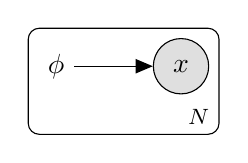
\begin{tikzpicture}
\node[obs] (x) {$ x $};
\node[left=of x] (phi) {$ \phi $};

\edge{phi}{x};

\plate {data} {(x)(phi)} {$ N $};
\end{tikzpicture}
}
\end{column}
\begin{column}{0.6\textwidth}
\alert{(Conditional) Density estimation}
\end{column}

\end{columns}

\begin{tabular}{p{2cm} p{4cm} p{4cm}}
 & Side information ($\phi$) & Observation ($x$) \\
Parsing &   \textcolor{gray}{a sentence} & \textcolor{black}{its syntactic/semantic parse tree/graph} \\
&&\\
Translation &  \textcolor{gray}{a sentence} & \textcolor{black}{its translation} \\
&&\\
Captioning &  \textcolor{gray}{an image} & \textcolor{black}{caption in English} \\
&&\\
Entailment  & \textcolor{gray}{a text and hypothesis} & \textcolor{black}{entailment relation}
\end{tabular}
\end{small}

\end{frame}

\begin{frame}{Where does deep learning kick in?}

Let $\phi$ be all side information available\\
~ e.g. deterministic \emph{inputs/features}

~

Have neural networks predict parameters of our probabilistic model
	\begin{align*}
    X|\phi \sim \Cat(\pi_{\alert \theta}(\phi)) & & \text{or} & & X|\phi \sim \mathcal N(\mu_{\alert \theta}(\phi), \sigma_{\alert \theta}(\phi)^2)
    \end{align*}
~ and proceed to \alert{estimate parameters} $w$ of the NNs %via MLE % that assign maximum likelihood to observations

 





\end{frame}



\begin{frame}{Task-driven feature extraction}

Often our side information $\phi$ is itself some high dimensional data
\begin{itemize}
	\item $\phi$ is a sentence and $x$ a tree
	\item $\phi$ is the source sentence and $x$ is the target
	\item $\phi$ is an image and $x$ is a caption
\end{itemize}
and part of the job of the NNs that parametrise our models is to also \alert{deterministically} encode that input in a low-dimensional space

%~
%\begin{itemize}
%	\item NNs parameterise probability functions
%	\item NNs predict parameters of a probabilistic model
%\end{itemize}

\end{frame}


\begin{frame}{NN as efficient parametrisation}

From the statistical point of view NNs do not generate data\\
\begin{itemize}
	\item \alert{they parametrise distributions} that \\
	\emph{by assumption} govern data
	\item compact and efficient way to \alert{map from complex side information to parameter space}
\end{itemize}

\vspace{10pt}

\pause
Prediction is done by a decision rule outside the statistical model
\begin{itemize}
	\item e.g. beam search
\end{itemize}

\end{frame}



\begin{frame}[plain]{Maximum likelihood estimation}

Let $p(x|\theta)$ be the probability of an observation $x$\\
~and $\theta$ refer to all of its parameters \\
~e.g. parameters of NNs involved

~ \pause

Given a dataset $x^{(1)}, \ldots, x^{(N)}$ of i.i.d. observations\pause

~

Log-likelihood function gives a criterion for parameter estimation
\begin{equation*}
\begin{aligned}
\mathcal L(\theta|x^{(1:N)}) &= \log \prod_{s=1}^N p(x^{(s)}|\theta) \\ \pause
 &= \sum_{s=1}^N \log p(x^{(s)}|\theta)
\end{aligned}
\end{equation*} 


\end{frame}

\begin{frame}[plain]{MLE via gradient-based optimisation}

If the log-likelihood is {\bf differentiable} and  {\bf tractable}\\
~then backpropagation can give us the gradient
\begin{small}
\begin{equation*}
\begin{aligned}
\grad_\theta \mathcal L(\theta|x^{(1:N)}) &= \grad_\theta \sum_{s=1}^N \log p(x^{(s)}|\theta) \\ \pause
 &=  \sum_{s=1}^N \grad_\theta \log p(x^{(s)}|\theta)
\end{aligned}
\end{equation*}
\end{small}  \pause

and we can update $\theta$ in the direction
\begin{equation*}
\gamma \grad_\theta \mathcal L(\theta|x^{(1:N)})
\end{equation*}
to attain a local maximum of the likelihood function

\end{frame}

\begin{frame}[plain]{Big Data}

For large \alert{$N$}, computing the gradient is inconvenient
\begin{small}
\begin{equation*}
\begin{aligned}
\grad_\theta \mathcal L(\theta|x^{(1:N)}) &=   \underbrace{\sum_{s=1}^{\alert{N}} \grad_\theta \log p(x^{(s)}|\theta)}_{\text{too many terms}} \\ \pause
&=   \sum_{s=1}^{\alert{N}} \textcolor{blue}{\frac{1}{ N} } N \grad_\theta \log p(x^{(s)}|\theta) \\ \pause
&= \sum_{s=1}^{\alert{N}}\textcolor{blue}{\mathcal U(s|\sfrac{1}{N})}  N \grad_\theta \log p(x^{(s)}|\theta) \\ \pause
&= \mathbb E_{S\sim \mathcal U(\sfrac{1}{N})}\left[ N \grad_\theta  \log p(x^{(S)}|\theta)\right]
\end{aligned}
\end{equation*} 
\end{small}
\pause

$S$ selects data points uniformly at random


\end{frame}

\begin{frame}[plain]{Stochastic optimisation}

For large $\alert{N}$, we can use a gradient estimate 
\begin{small}
\begin{equation*}
\begin{aligned}
\grad_\theta \mathcal L(\theta|x^{(1:N)}) 
 &=  \underbrace{\mathbb E_{S\sim \mathcal U(\sfrac{1}{N})}\left[ N \grad_\theta  \log p(x^{(S)}|\theta)\right]}_{\text{expected gradient :)}} \\ \pause
 &\overset{\text{MC}}{\approx} \frac{1}{M} \sum_{m=1}^M N  \grad_\theta \log p(x^{(s_i)}|\theta) \\
 &S_i \sim \mathcal U(\sfrac{1}{N})
\end{aligned}
\end{equation*}
\end{small}  \pause
and take a step in the direction
\begin{equation*}
\gamma \frac{N}{M} \grad_\theta \mathcal L(\theta|x^{(s_1:s_M)})
\end{equation*}
where $x^{(s_1:s_M)}$ is a random mini-batch of size $M$


\end{frame}




\begin{frame}{DL in NLP recipe}


%Vast majority of papers published at ACL

%\begin{small}
%\begin{figure}
%\scalebox{0.8}{
%\begin{tikzpicture}
%\node[obs] (x) {$ x $};
%\node[left=of x] (phi) {$ \phi $};
%\factor[left=of x] {f} {below:$f_w$} {phi} {x} ; 
%%\edge{phi}{x} ;
%\plate {data} {(x)(phi)} {$ N $};
%\end{tikzpicture}
%}
%\end{figure}
%\end{small}
	Maximum likelihood estimation
	\begin{itemize}
		\item  tells you which \alert{loss} to optimise \\
		(i.e. negative log-likelihood)
	\end{itemize}
	
	Automatic differentiation (\emph{backprop})
	\begin{itemize}
		\item ``give me a tractable forward pass and I will give you \alert{gradients}''
	\end{itemize}
	
	Stochastic optimisation powered by backprop
	\begin{itemize}
		\item general purpose gradient-based optimisers
	\end{itemize}

\end{frame}


\begin{frame}{Tractability is central}

Likelihood gives us a differentiable objective to optimise for
\begin{itemize}
	\item but we need to stick with \alert{tractable} likelihood functions
\end{itemize}



%, any intractable likelihood will leave us in bad territory because
%\begin{itemize}
%	\item stochastic optimisation requires gradient estimates
%	\item which must be unbiased (forget greedy techniques)
%	\item and some estimation techniques are not differentiable (forget MC sampling)
%\end{itemize}

\end{frame}


\begin{frame}{When do we have intractable likelihood?}

{\bf Unsupervised problems} contain unobserved random variables\\ 
\begin{equation*}
p(x, z|\theta) = \overbrace{p(z)}^{\text{prior}} \underbrace{p(x|z, \theta)}_{\text{observation model}}
\end{equation*}

~ \pause

thus assessing the marginal likelihood requires \alert{marginalisation of latent variables} 
\begin{equation*}
p(x|\theta) = \int p(x, z|\theta) \dd{z} = \int p(z)p(x|z, \theta) \dd{z} 
\end{equation*}

\end{frame}


\begin{frame}{Examples of latent variable models}

Discrete latent variable, continuous observation
	\begin{small}
	\begin{equation*}
	p(x|\theta) = \underbrace{\sum_{c=1}^K \Cat(c|\pi_1, \ldots, \pi_K) \underbrace{\mathcal N(x|\mu_\theta(c), \sigma_\theta(c)^2)}_{\text{forward pass}}}_{\text{{\bf too many forward passes}}}
	\end{equation*}
	\end{small} 

	\pause
	
Continuous latent variable, discrete observation
	\begin{small}
	\begin{equation*}
	p(x|\theta) = \underbrace{\int \mathcal N(z|0, I) \underbrace{\Cat(x|\pi_\theta(z))}_{\text{forward pass}} \mathrm{d}z }_{\text{\alert{{\bf infinitely many forward passes}}}}
	\end{equation*}
	\end{small}

\end{frame}


\begin{frame}{But why latent variable modelling?}

Some reasons

\begin{itemize}
	\item organise a massive collection of data\\
	e.g. LDA	 \pause
	\item learn from unlabelled data\\
	e.g. semi-supervised learning \pause
	\item learn from little data\\
	e.g. Bayesian NNs \pause
	\item induce discrete representations\\
	e.g. parse trees, dependency graphs, permutations, alignments
	%e.g. derivatives are not defined for discontinuous functions
\end{itemize}

\end{frame}


\begin{frame}{Deep Generative Models}

Probabilistic models parametrised by neural networks
\begin{itemize}
	\pause
	\item explicit modelling assumptions\\
	one of the reasons why there's so much interest	
	\pause
	\item but requires efficient inference\\
	\pause
	\alert{which is the reason why we are here today}
\end{itemize}

\end{frame}

\end{document}
